\chapter{State of the Art}
\label{cha:state of the art}

\section{Automated and Autonomous Vehicles}

This thesis aims to increase the autonomy of mobile robots. In order to define an improvement in autonomous behavior, one needs to explore the definitions of the terms "automated" and "autonomy". The "Expertenkommission Forschung und Innovation" (EFI) defines the term autonomy in the context of robotics as a system that can act without human instructions and still solve complex tasks, make decisions, learn independently as well as react to unforeseen circumstances \cite{efi2018}. The definition specifies the needed requirements to make a robot fully autonomous.

\begin{figure}[ht]
	\centering
	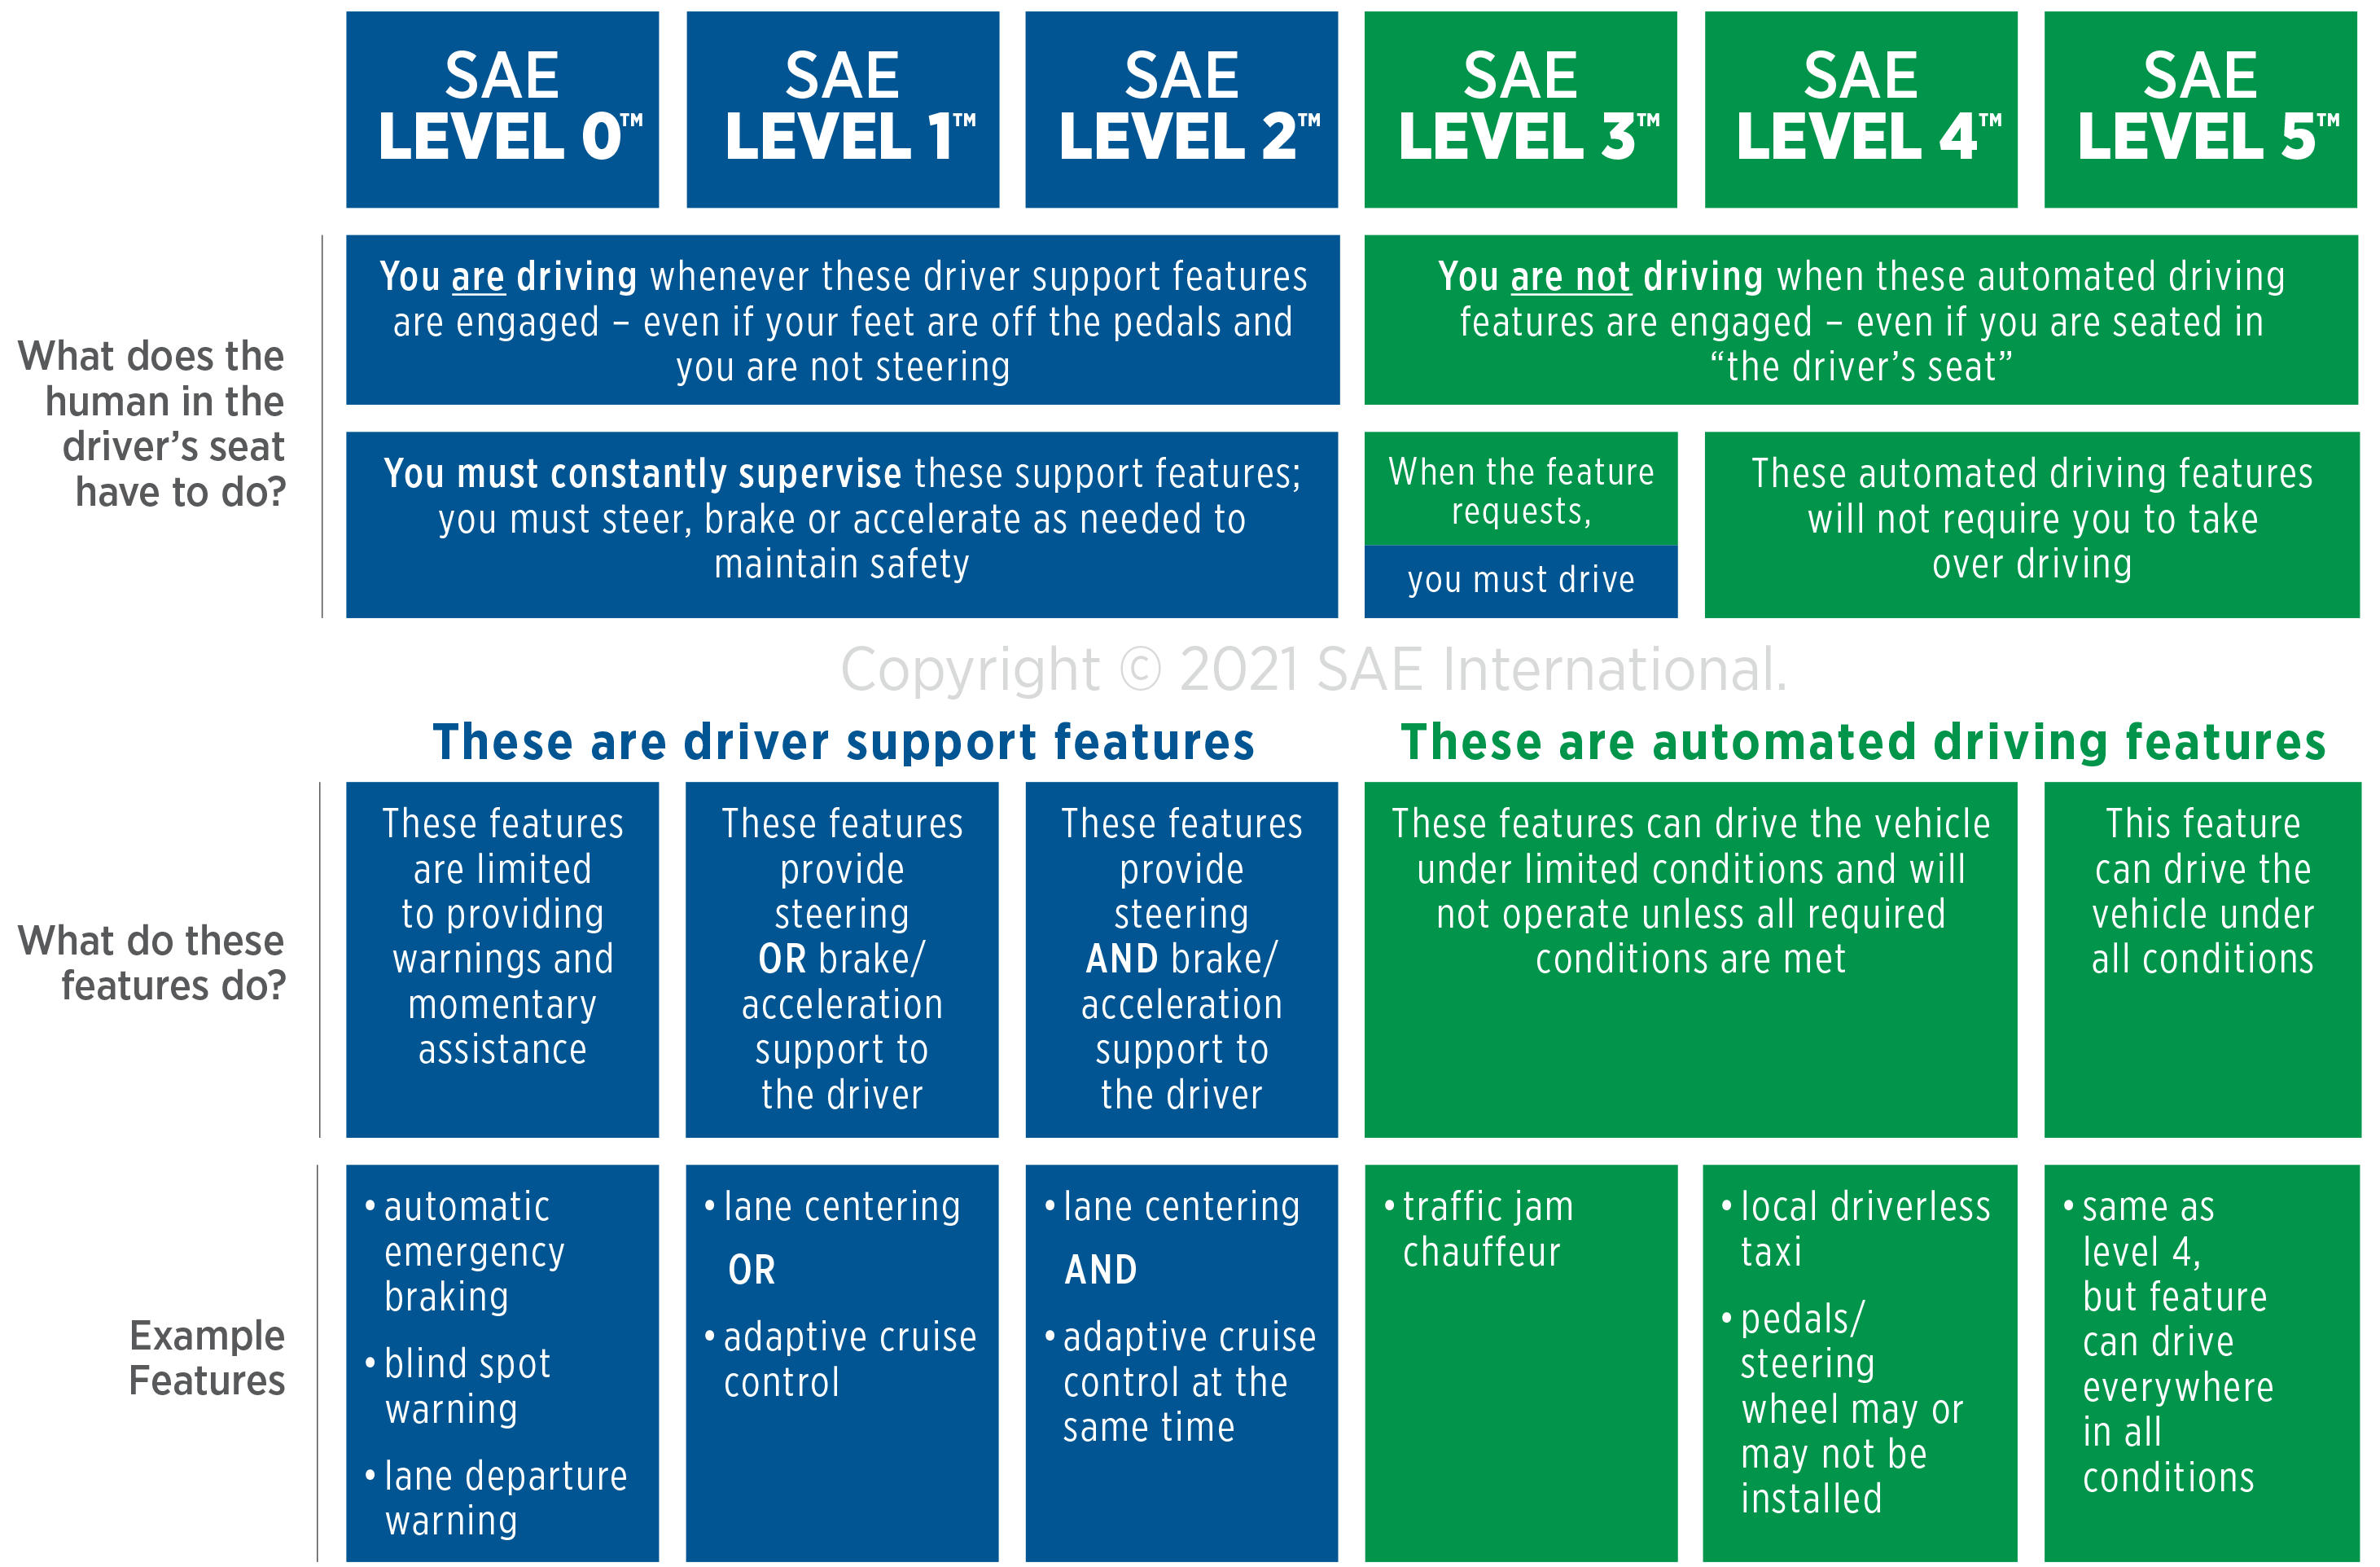
\includegraphics[width=0.9\textwidth]{images/j3016graphic_2021.png}
	\caption{Levels Of Driving Automation \cite{J3016_202104}}
	\label{fig:sae_levels}
\end{figure}

The Society of Automotive Engineers (SAE) defines vehicle autonomy based on the human driver's need for supervision and possible intervention when executing complex driving tasks \cite{J3016_202104}. Figure \ref{fig:sae_levels} depicts the different levels of autonomy of passenger cars on a scale between no automation to completely autonomous. The most significant distinction between the levels is between level two and three, because a system can take the complete control over the vehicle in certain conditions. The SAE levels zero to two use driver support functions with no real autonomy, while levels three to five employ automated driving features.
Another major level difference is located on the borderline between levels three and four as the vehicle can drive autonomously without a human operator who could control the vehicle as a safety fallback when the system demands it. A level four vehicle can theoretically be built without a steering wheel and pedals, because it is able to handle all situations it is deployed in without the need for manual driving. 
%The most significant distinction between the levels is between level three and four, because a vehicle can drive without a human driver as a safety fallback option. 

Both definitions rely on human supervision and guidance as the central part of what hinders a system or vehicle from becoming fully autonomous. By decreasing the instances of human intervention during the operation of a robot, one can increase the automation level towards full autonomy. However, this has to be done by equipping the robot with robust and context-driven decision-making and planning capabilities. Otherwise, a robot that never needs a human to operate could easily be created. Nevertheless, this robot could not be considered autonomous as it would not be able to solve complex tasks and make intelligent decisions.

%Different levels of autonomy require different methodologies to achieve them. 

%SAE Levels
%EFI Gutachten
%Fachforum 

\section{Autonomous Driving Navigation Architectures}
\label{sec:Autonomous Driving Navigation Architectures}

To better understand how behavior planning influences a robot's autonomy, one can look at the latest and most used software architectures for autonomous driving on a functional level. The majority of the current autonomous driving architectures implement a hierarchical structure that follows the "\textit{Sense - Think - Act}" paradigm \cite{murphy2000}. 

\begin{figure}[ht]
	\centering
	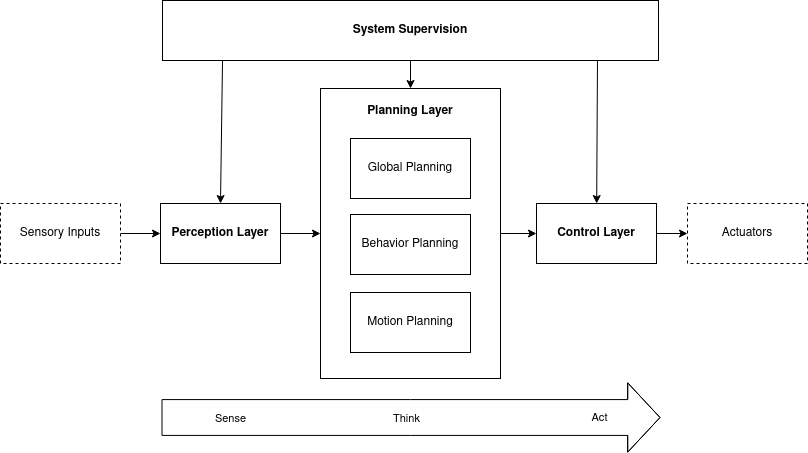
\includegraphics[width=0.9\textwidth]{images/autonomous_driving_architecture.png}
	\caption{Common Autonomous Driving Architecture \cite{brooks1986,velasco2020}}
	\label{fig:autonomous_driving_architecture}
\end{figure}

As shown in figure \ref{fig:autonomous_driving_architecture}, the sensory inputs, usually from multiple sensors, are processed to create an environment representation. Based on that representation, the system calculates how to get from its current position to the destination and creates a path to the destination. A second planning calculation is triggered to compute the motion commands while taking the system's constraints (e.g., size, turning radius) into account. In a final step, these motion commands then get converted to control the motors. 

The planning sequence can be further divided into "$global$", "$behavioral$", and "$local$" planning. The global planning module, also named "$route$ $planning$", is responsible for outputting a path from start to goal. Global planning is comparable to a person using Google Maps to find the shortest or fastest path to a faraway city. In this analogy, the behavior planner is responsible for following the traffic rules on the trip to the destination, e.g., stopping at red lights, giving the right of way to other vehicles, and following speed limits. The local planning, also named motion planning, takes the input from the behavior layer and is tasked to let the vehicle drive according to the executed behavior so that it stays in its lane and stops at a red light at the correct position \cite{reke2020}.

Due to safety considerations, many autonomous driving architectures implement an additional system supervision layer that monitors the execution of the other system components. This supervisor checks the health of all software components. If one or more components fail to pass the health check, the supervisor is responsible for ensuring that the system does not continue the regular driving routine. The supervision component triggers measures to restore the standard functionality or, if that is not possible, bring the robot into a safe state \cite{zimmermann2020adaptive}.

Considering that with these architectures, vehicles can achieve an SAE level of autonomy up to level four and even five \cite{bacha2008odin}, a good starting point to increase autonomy in a robotic system would be to ensure that all of the functional modules in figure \ref{fig:autonomous_driving_architecture} are implemented and available. Based on this, higher autonomy levels are achievable by expanding the behavior planning module inside the planning layer. 

%bacha2008
%reke 2020
%wei2014
%brooks1986
%dhillon 2002
%gonzales2016

\section{Behavior Types}
\label{sec:Behavior Types}

The behavior planning module contains a set of tailored behaviors to operate in a specific environment. The module's task is to always choose the best behavior to execute to ensure the best performance for a given task. In this sense, behavior is defined as a mapping of sensory inputs to a pattern of actions that carry out a specific task \cite{murphy2000}. A good behavior planning approach provides the robot with acceptable behaviors for every possible scenario the robot is operating in. Different scenarios pose different challenges for the behavior planning module, which has to decide on the best behavioral option to achieve a higher-level goal. 

\subsection{Reactive}

During the emergence of behavior-based robots in the 1960s, the first type of behaviors implemented were simple reactive behaviors. This behavior type maps a sensory input directly to motor commands. In human behavior, this behavior resembles reflexes, like tapping on the kneecap, which unwillingly results in motion in the knee joint. This behavior pattern is not following the typical "Sense, Think, Act" loop, but shortcuts directly from sensing to acting \cite{desilva2008}. Reactive behaviors can be chained together to achieve more advanced and goal-driven behaviors. 

Despite the possibility to carry out more complex robot behaviors, sequential behaviors remain largely on the level of reactive behaviors due to the lack of a planning and decision-making cycle during their execution. The computational load of reactive behaviors is low and therefore fast as no decision and planning process is taking place, which makes them suited in scenarios where real-time safety is of concern. This property makes this behavior type useful for system supervisors, where immediate reactions with low latency are sometimes required to ensure system safety. 

However, a system with a solely reactive behavior planning approach will always fail to meet the requirements for higher levels of autonomy due to the reasons discussed in previous chapters. This systematic lack of autonomy does not mean reactive behaviors can not be part of highly autonomous systems. The quick response time to sensor inputs makes them valuable in improving vehicle safety and reliability. 

\subsection{Deliberative}

Systems purely based on reactive behaviors suffer the drawback that they do not allow for complex behaviors. In addition, creating sequences of reactive behaviors that produce the target behavior is a complicated task \cite{murphy2000}. Behaviors that involve planning and decision-making aspects are defined as deliberative. Unlike reactive behaviors, deliberative behaviors follow the "\textit{Sense - Think - Act}" paradigm, and they are not mapping sensory inputs directly into motor commands. Instead, deliberative-type behaviors can decide the best course of action before they act. Using deliberative behaviors inside of the planning module enables a robot to meet the definition of autonomy, especially in regards to the making of decisions and reacting to unforeseen circumstances. 

A behavior planner with a deliberative approach can make decisions based on current sensor data and previously processed data. By incorporating older sensor information into the decision-making process, the deliberative behavior planner can predict changes in the environment. Using older data points allows the planner to proactively adapt the motion planning commands to better achieve goals in dynamic and uncertain environments. 

For example, a motion prediction of obstacles in highly dynamic environments would improve motion planning considerably. The behavior planner can adjust the motion planning with more precise information on how dynamic obstacles interact with the robot's planned path in the future. A purely reactive planner could never determine if an obstacle is destined to intersect the robot's path in the future and would constantly reroute to accomplish the given goal.

On the other hand, a deliberative planner can determine if the best course of action is to stay on the current path as the dynamic obstacle has already moved away by the time the robot reaches the intersection point. Other actions in the scenario are possibly slowing down or speeding up briefly to avoid an obstacle and staying on the current path, which is calculated to be quicker than rerouting and taking a longer path. 


Concluding, the focus should be on creating deliberative behaviors to improve autonomy. Generally, these cognitively more complex behaviors mimic human skills and thus make a system more autonomous, because the need for a human operator can be decreased greatly.

%\textit{Talk about machine learning as deliberative behavior -> true autonomy bc learning and unknown scenarios, programmers can not cover every scenario, so a well designed/trained ai is needed to make a system really autonomous, but -> missing determinism and unaccountability of machines, hence we need behaviors that are still hard coded and deterministic, these can be highly automated. traditional behaviour and ai generated behaviours can and must coexist in the system (adler2019)}
%
%silva2008
%ingrand 2014
%vasiolopolous 2022

\subsection{Hybrid}

One can combine reactive and deliberative behaviors in a hybrid model to create reliable and intelligent systems. This behavior planning module can quickly react to incoming sensor data and still exhibit high levels of automation. 

\begin{figure}[ht]
	\centering
	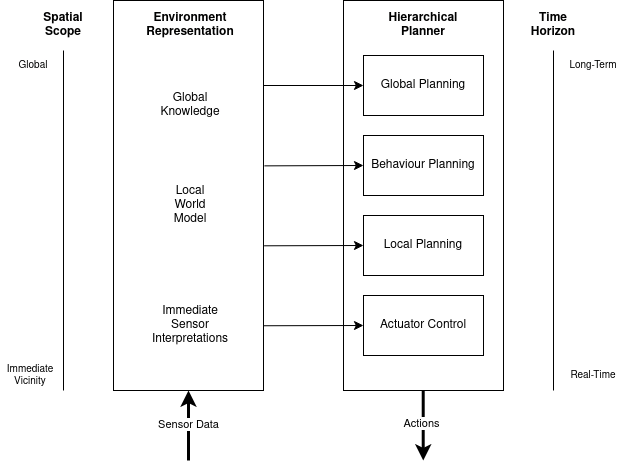
\includegraphics[width=0.9\textwidth]{images/Deliberative_hierarchical_planning.png} 
	\caption{Hybrid Planning Architecture \cite{arkin1998}}
	\label{fig:hybrid_planning}
\end{figure}

Figure \ref{fig:hybrid_planning} shows the areas where reactive and deliberative behaviors have advantages and limitations. Deliberative planning does possess limitations during the execution of generated plans as the time horizon is long-term and not able to react to fast changes in the environment. When the system is not addressing these points, deliberative robots are very focused on a narrow problem domain and are not robust when the defined system boundaries are crossed\cite{arkin1998}.

The incorporation of reactive behaviors into behavior planning combats this problem. In this multi-layer approach, the higher level, more deliberative planners can override the reactive planners to allow the system to be more flexible in uncertain environments and adaptable while maintaining fast reaction times. This architecture leads to more robust robots deployed in a wider variety of environments, thus leading to higher levels of autonomy.

\section{Behavior Planning Approaches}
\label{sec:Behavior Planning Approaches}

Robots that use a hybrid, hierarchical behavior planning approach need a system that decides on a high level which behaviors are executed. That system allows overriding simple reactive behaviors with more complex, deliberative behaviors when the whole system benefits from them. 

The solutions for behavior execution systems, presented in the following sections, all share the usage of states that a robot can be in. Different strategies and behaviors are utilized during the system's runtime based on a robot's state and additional information about the environment. 
 
In the following sections, different approaches for behavior planning are presented and compared.

\subsection{Finite State Machines}

Finite State Machines (FSM) are commonly used in the autonomous driving domain. They describe behavior in the form of states, which trigger the execution of actions. A finite state machine is defined by a list of possible states \textit{}, a starting state $s_{0}$, a set of state transitions $\delta$, a set of final states $F$, and the input alphabet $\sigma$. At any given time, only a single state is selected, and its containing actions are executed. 

Figure \ref{fig:fsm} depicts an example state machine with different states and exemplary transitions between them. Inside of the states the letters indicate the existence of actions. $E$ stands for entry, $I$ for Input and $X$ for Exit. The arrows between the states illustrate the possible transition and transition conditions for every state. A state transition diagram is an excellent way to understand the system behavior, but can not show the details of the modeled behavior, like the actions \cite{wagner2006}. 

\begin{figure}[ht]
	\centering
	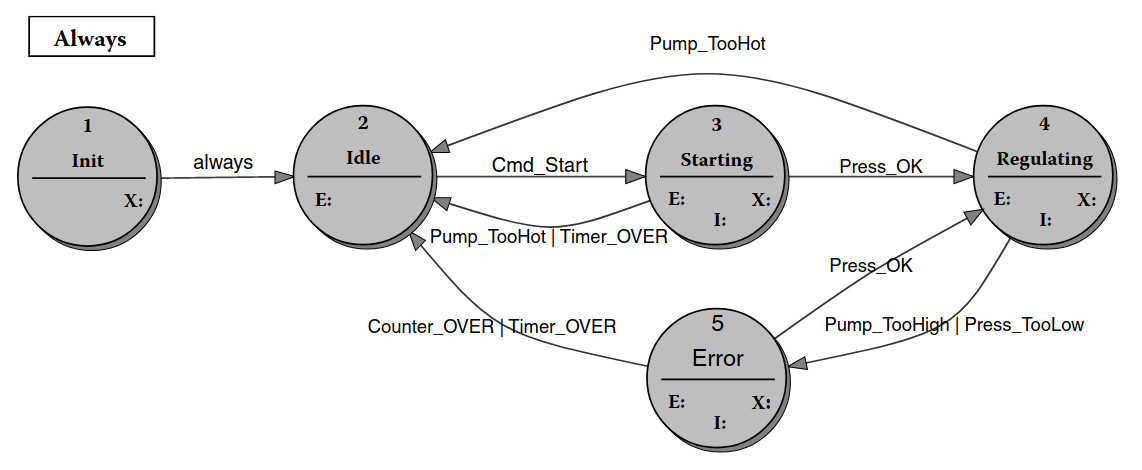
\includegraphics[width=0.9\textwidth]{images/fsm.png} 
	\caption{Example of a finite state machine transition diagram \cite{wagner2006}}
	\label{fig:fsm}
\end{figure}

The execution time of finite state machines can be fast enough to control the motors of a bipedal robot to enable the robot to balance and walk despite unexpected height variations between steps \cite{park2013}. The high performance makes state machines very well suited for fast, reactive type behaviors while still allowing a deliberative and hierarchical approach to behavior planning.

Creating small state machines can be accomplished easily and quickly using various feature-rich and performant libraries \cite{fourakis2014}. Finite state machines are often used to model reactive and sequential behaviors comprehensively in autonomous driving functions \cite{ziegler2014}. These finite state machines use nested state machines inside another state machine. The nested state machines reduce the complexity of the state machine as the transitions do not need to be modeled because a nested state machine's start and final state are treated as just one state inside the bigger state machine. 

Despite the possibility of nesting state machines, the effort to expand and maintain a FSM multiplies rapidly, when the system becomes increasingly larger to integrate more complex behaviors. The higher effort is due to the required creation of the transitions, transition conditions, and transition events. The FSM needs to be updated with each new state that gets introduced into the state machine as existing states need to be checked and corrected accordingly \cite{conner2017}. 
%
%allgeuer 2013
%connor 2017
%ziegler 2014

\subsection{Behavior Trees}
\label{subsec:Behavior Trees}

Behavior Trees (BT) are another way to model and control the behavior of autonomous systems. Behavior Trees first found considerable acceptance in the computer game industry, where they are mainly used to model artificial intelligence for non-player characters \cite{florez2009}. Every tree has one root and many children, parent, and leaf nodes. Leaf nodes are also called execution or action nodes, while non-leaf nodes are control or control flow nodes. 

\begin{table}[ht]
	\centering
	\caption{The five types of behavior tree nodes \cite{iovino2022}}
	\label{tab:node_types}
	\renewcommand{\arraystretch}{1.5}
	\resizebox{0.9\textwidth}{!}{%
		\begin{tabular}{ | m{0.13\textwidth} | m{0.13\textwidth}| m{0.2\textwidth} | m{0.2\textwidth} | m{0.2\textwidth} |} 
	 	\hline
	 	\textbf{Node type} & \textbf{Symbol} & \textbf{Succeeds} & \textbf{Fails} & \textbf{Running} \\ 
	 	\hline
	 	Sequence & -$>$ & If all children succeed & If one child fails & If one child returns running \\ 
	 	\hline
	 	Fallback & ? & If one child succeeds & If all children fail & If one child returns running \\ 
	 	\hline
	 	Parallel & -$>$ -$>$ & If $>=$ M children succeed & If $>$ N-M children fail & else \\
	 	\hline
	 	Action & shaded box & Upon completion & If impossible to complete & If node is still completing tasks \\
	 	\hline
	 	Condition & white oval & If true & If false & Never \\
	 	\hline
		\end{tabular}
	}
\end{table}

The execution of a behavior tree is done by ticking the tree's root node. This signal then travels down to the child node of the root node, where either control nodes are ticked, or action nodes are executed. Nodes return either "Success", "Running" or "Failure" which influences how the tick signal gets processed by the rest of the behavior tree. 

The relevant control nodes are of the type "Sequence", "Fallback" or "Condition". The condition node can not have child nodes and can only return success or failure. A sequence node can be compared to a logical "and" condition. This property of the sequence node means that once a sequence gets ticked from the parent node, it will send the tick signal to every child node as long as they return "Success" or "Running" and only return "Success" itself when every child node was successfully ticked. If any children nodes return "Failure", the sequence node will stop ticking the remaining children and return "Failure".

On the other hand, the fallback node is an equivalent of a logical "Or" condition. The fallback node ticks its children nodes as long as they return "Failure" or "Running" and will return "Success" if one of the ticked nodes returned "Success". It will only return "Failure" if all children nodes returned "Failure". The primary node types and their control flow modification are listed in table \ref{tab:node_types}. Parallel control nodes are listed for completeness, but are not discussed further in this chapter due to their limited use in robotic applications.

Figure \ref{fig:bt_example} depicts an example of a BT with multiple levels and action nodes. The nodes with the arrow (-$>$) symbol are sequence nodes, and the question mark ($?$) symbol denotes fallback nodes. The condition nodes are depicted as white ovals, and the action nodes are represented as gray rectangles in the behavior tree example.

\begin{figure}[ht]
	\centering
	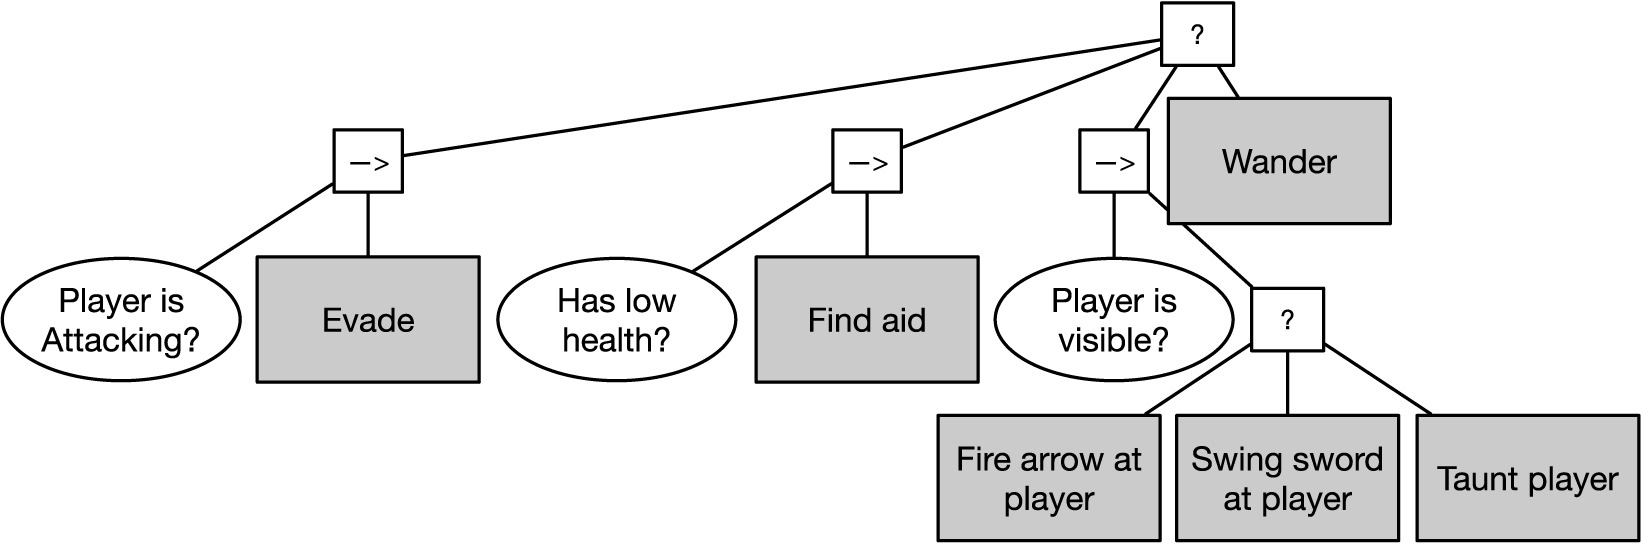
\includegraphics[width=0.9\textwidth]{images/bt_example.jpg} 
	\caption{Example of a behavior tree \cite{iovino2022}}
	\label{fig:bt_example}
\end{figure}

One of the core differences to the Finite State Machine is that transitions between states are not distributed across all the states. In contrast, they are organized in a hierarchical tree, where the leaves represent the states \cite{iovino2022}. FSM and BT can produce the same behavior in robots. However, the fundamental shift in how the two systems are created leads to significant advantages in the modularity, synthesis, and analysis of the systems at hand. These effects are more significant with an increase in the size of the system. Behavior trees offer much more flexibility when creating an advanced behavior layer for an autonomous system. 

%iovino2022
%marzinotto 2014
%colledanchise 2018

\subsection{Partially Observable Markov Decision Processes}

Another approach to behavior planning is the Markov Decision Process (MDP) and the further advanced Partially Observable Markov Decision Process (POMDPs). MDPs share structural features with Finite State Machines, but the behavior planning and state transitions are stochastic and not deterministic in contrast to FSMs. An MDP can be described as a tuple $<S, D, A, T, R>$. Like a finite state machine, the MDP has a set of possible states \textit{S} and a set of possible transitions \textit{T} between them. The transitions contain a probability of execution and must add up to 1.0 for each associated state. An MDP adds a set of finite actions \textit{A} and rewards \textit{R} to the system. Additionally, MDPs possess a set of discrete time steps, in this context often called epochs, \textit{D}, which can be infinitely long. The guiding principle of MDPs is to maximize the expected reward by deciding on the best action. This policy $\pi$ is what guides the behavior of the MDP \cite{feyzabadi2014riskaware}.

\begin{figure}[ht]
	\centering
	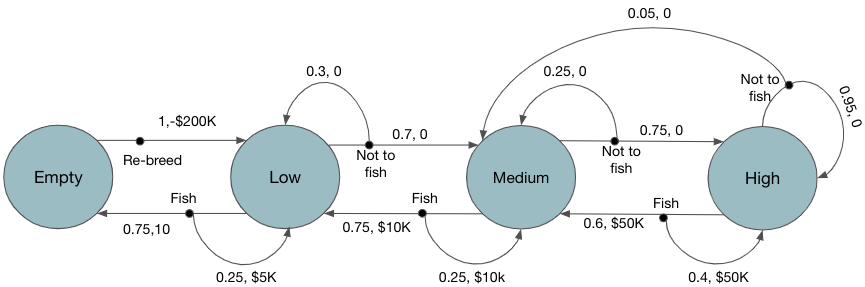
\includegraphics[width=0.9\textwidth]{images/mdp.png} 
	\caption{Example of a fully observable Markov Decision Process \cite{andrew1999reinforcement, banerjee2021real}}
	\label{fig:mdp}
\end{figure}

Figure \ref{fig:mdp} shows an exemplary MDP for determining a fisherman's best course of action. The states are the population sizes of available fish, and the only available actions are to either fish or not to fish. The actions possess different rewards depending on the current state of the system \cite{tanwar2019markov}. 

The difference between an MDP and a POMDP is that in a POMDP the system's current state can be unknown, and the system can make observations and estimate the state to a degree. The POMDP is defined as a tuple $<S, D, A, T, R, Z, O>$ in which the MDP tuple gets extended by \textit{Z} and \textit{O}. \textit{Z} is the observation, and \textit{O} is the probability function of seeing \textit{Z} in a given state \textit{S}.

POMDPs are well suited for applications in unknown environments because the system can make decisions if the perception information is imperfect, or the environment is not fully observable. The decision process is probabilistic and is more adaptable when confronted with unknown scenarios. This flexibility comes at the cost of determinism. The system's behavior is not guaranteed to be the same whenever it is subjected to the same sensory input \cite{krishnamurthy2016partially}.

% \section{Deterministic Behavior}
